\chapter{Analiza și proiectarea sistemului}

\section{Pornirea de la cerințe}

Înaintea implementării funcționalităților principale, a fost necesară separarea cât mai clară a cerințelor sistemului. Pentru acest tip de proiect, riscul cel mai mare este adăugarea multor funcții atractive, dar fără o structură clară. De aceea, analiza a pornit de la întrebarea simplă: ce trebuie să poată face utilizatorul și ce trebuie să poată susține sistemul în spate?

Din perspectiva utilizatorului final, aplicația trebuie să permită crearea unui cont, autentificarea, administrarea profilului, lucrul cu proiecte și folosirea editorului vizual. Din perspectiva fluxului de produs, trebuie să existe și operații precum publicarea unui proiect, explorarea proiectelor altora, aprecierea lor și reutilizarea prin fork. Din perspectiva obiectivului tehnic al lucrării, sistemul trebuie să poată genera designuri cu ajutorul AI și să exporte rezultatul în cod.

Aceste cerințe au fost apoi grupate în două categorii mari: funcționale și nefuncționale.

\section{Cerințe funcționale}

Principalele cerințe funcționale identificate pentru Favigon sunt următoarele:

\begin{enumerate}[leftmargin=1.5cm]
  \item utilizatorul poate crea cont, autentifica și ieși din aplicație;
  \item utilizatorul poate folosi login clasic sau autentificare prin furnizori externi;
  \item utilizatorul poate activa sau dezactiva autentificarea în doi pași;
  \item utilizatorul își poate edita profilul și imaginea de profil;
  \item utilizatorul poate crea, edita și șterge proiecte;
  \item pentru fiecare proiect, utilizatorul poate salva designul și thumbnail-ul asociat;
  \item utilizatorul poate edita vizual proiectul într-un canvas cu mai multe pagini;
  \item utilizatorul poate genera o structură de design prin AI, inclusiv în regim streaming;
  \item utilizatorul poate valida și exporta proiectul în HTML, React sau Angular;
  \item utilizatorul poate marca proiectele altora cu like sau star;
  \item utilizatorul poate urmări alți utilizatori și poate vedea proiecte recomandate;
  \item utilizatorul poate fork-ui proiecte publice și le poate adapta în propriul spațiu.
\end{enumerate}

La nivel de implementare, aceste cerințe se reflectă destul de direct în controllerele și serviciile backend, respectiv în feature-urile frontend. De exemplu, `AccountController` și `AuthService` acoperă fluxurile de autentificare, `ProjectsController` și `ProjectService` gestionează ciclul de viață al proiectelor, iar `AiDesignController` împreună cu serviciile AI acoperă generarea asistată. Pentru a păstra legătura dintre obiective, module și validare, Tabelul~\ref{tab:trasabilitate-obiective} sintetizează corespondențele principale.

\section{Cerințe nefuncționale}

Pe lângă cerințele funcționale, proiectul are și câteva cerințe nefuncționale importante:

\begin{itemize}[leftmargin=1.5cm]
  \item \textbf{claritate arhitecturală}: logica de business nu trebuie amestecată în controllere;
  \item \textbf{extensibilitate}: exportul către mai multe framework-uri trebuie să fie posibil fără rescrierea editorului;
  \item \textbf{performanță interactivă}: editorul trebuie să rămână fluid pentru operațiile uzuale;
  \item \textbf{siguranță}: autentificarea și operațiile sensibile trebuie protejate rezonabil;
  \item \textbf{persistență robustă}: designul proiectelor trebuie salvat automat și recuperat coerent;
  \item \textbf{portabilitate}: aplicația trebuie să poată fi pornită ușor local și demonstrată într-un mediu apropiat de producție;
  \item \textbf{testabilitate}: cel puțin partea de backend și motorul de conversie trebuie să poată fi verificate prin teste automate.
\end{itemize}

Aceste cerințe nefuncționale au influențat puternic structura aplicației. Necesitatea de a exporta în mai multe tehnologii a dus aproape inevitabil la introducerea reprezentării intermediare. Necesitatea de a păstra editorul fluid a dus la împărțirea logicii în servicii specializate pe frontend. Necesitatea de a limita amestecul de responsabilități a dus la structurarea backend-ului pe straturi.

\begin{table}[H]
  \centering
  \caption{Trasabilitatea dintre obiectivele proiectului, module și validare}
  \label{tab:trasabilitate-obiective}
  \renewcommand{\arraystretch}{1.15}
  \begin{tabularx}{\textwidth}{>{\RaggedRight\arraybackslash}p{4.2cm}YY}
    \toprule
    \textbf{Obiectiv} & \textbf{Module principale} & \textbf{Formă de validare} \\
    \midrule
    Autentificare și administrare cont & `AccountController`, `AuthService`, `UsersController` & teste backend pentru autentificare și scenarii funcționale de login / 2FA \\
    Editor vizual multi-page & `CanvasPage`, `CanvasEditorStateService`, `CanvasPageManagerService` & scenarii de editare, autosave și restaurare de stare \\
    Reprezentare intermediară reutilizabilă & mapper-e canvas $\leftrightarrow$ IR, `IRNode`, `ConverterService` & validare structurală înainte de export și teste pentru convertor \\
    Generare asistată de AI controlabilă & `AiDesignController`, `AiDesignService`, `AiPipelineService`, `OpenAiClient` & validare structurală, mecanism de auto-reparare și scenarii funcționale AI \\
    Export multi-framework & `ConverterController`, `ConverterService`, `ConverterEngine` & teste pentru HTML / React / Angular, responsive și multi-page \\
    Componentă socială și reutilizare & `ProjectsController`, `UsersController`, `ExploreController`, `ProjectService` & teste service/controller și scenarii de publicare, like, star și fork \\
    \bottomrule
  \end{tabularx}
\end{table}

\section{Actorii principali}

Sistemul are două categorii principale de actori.

\textbf{Utilizatorul neautentificat} poate accesa paginile publice, poate vedea proiectele expuse și poate explora conținutul public. El nu poate modifica proiecte și nu poate folosi editorul complet.

\textbf{Utilizatorul autentificat} reprezintă actorul central al sistemului. Acesta își poate administra profilul, își poate crea și edita proiectele, poate folosi editorul canvas, poate apela generarea AI, poate exporta cod și poate interacționa social cu alți utilizatori.

Pentru a sintetiza relația dintre actori și funcționalitățile dominante, Figura~\ref{fig:use-case-favigon} prezintă o vedere de tip use-case. Ea nu urmărește toate endpoint-urile sau toate stările posibile, ci capabilitățile care structurează produsul la nivel de utilizare.

\begin{figure}[H]
  \centering
  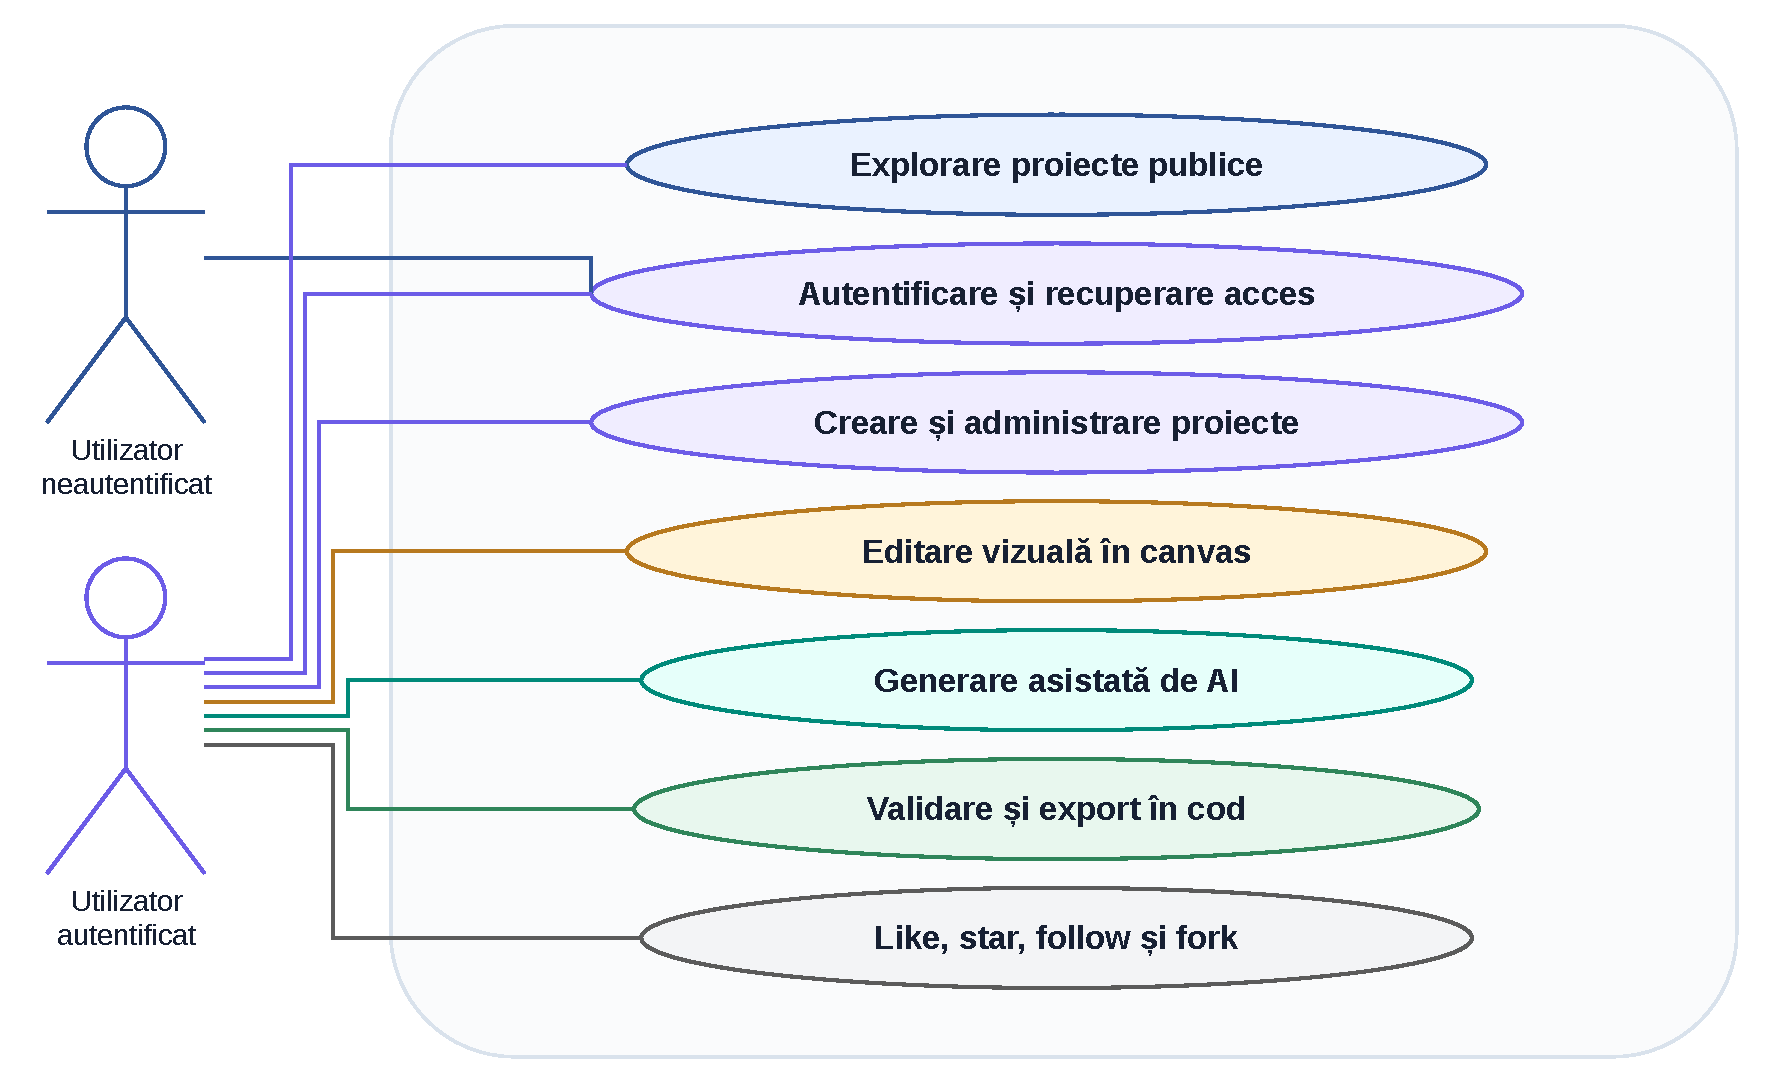
\includegraphics[width=0.97\textwidth]{diagrams/use-case-favigon.drawio.pdf}
  \caption{Diagrama de use-case simplificată pentru funcționalitățile principale din Favigon}
  \label{fig:use-case-favigon}
\end{figure}

\section{Scenarii principale de utilizare}

\subsection{Scenariul 1: creare și editare proiect}

Utilizatorul se autentifică, creează un proiect nou și ajunge în editorul canvas. Acolo poate adăuga elemente, poate crea pagini noi, poate modifica proprietăți și poate salva implicit progresul. La ieșire sau la schimbarea paginii, sistemul trebuie să se asigure că starea relevantă este persistată.

\subsection{Scenariul 2: generare asistată de AI}

Utilizatorul pornește de la un prompt și solicită generarea unei interfețe. Backend-ul trimite cererea către serviciul AI, primește etapele pipeline-ului și returnează rezultatul. Frontend-ul transformă structura obținută în elemente de canvas și permite utilizatorului să continue editarea manuală. Acest scenariu este important deoarece arată că AI-ul este integrat în fluxul editorului, nu separat de el.

\subsection{Scenariul 3: export în cod}

După ce proiectul ajunge într-o stare satisfăcătoare, utilizatorul cere validarea și exportul. Designul este convertit în reprezentarea intermediară, verificat și transmis motorului de conversie. Rezultatul este un set de fișiere pentru framework-ul ales. Acest scenariu justifică existența convertorului ca modul separat.

\subsection{Scenariul 4: distribuire și reutilizare}

Un utilizator publică un proiect, iar alt utilizator îl descoperă în explore sau pe profilul autorului. Poate să îl aprecieze, să îl salveze sau să îl fork-uiască. În acest fel, proiectul capătă și o dimensiune de comunitate, nu rămâne doar un document privat.

\section{Arhitectura generală}

La nivel înalt, sistemul este împărțit în frontend, backend, bază de date și servicii externe. Frontend-ul Angular gestionează interfața, rutarea și starea locală a editorului. Backend-ul ASP.NET Core expune endpoint-uri REST și coordonează logica de aplicație. PostgreSQL stochează datele persistente. Serviciile externe includ OpenAI API pentru generare și Cloudflare Tunnel pentru expunere controlată. Arhitectura logică rezultată este redată în Figura~\ref{fig:arhitectura-generala}.

\begin{figure}[H]
  \centering
  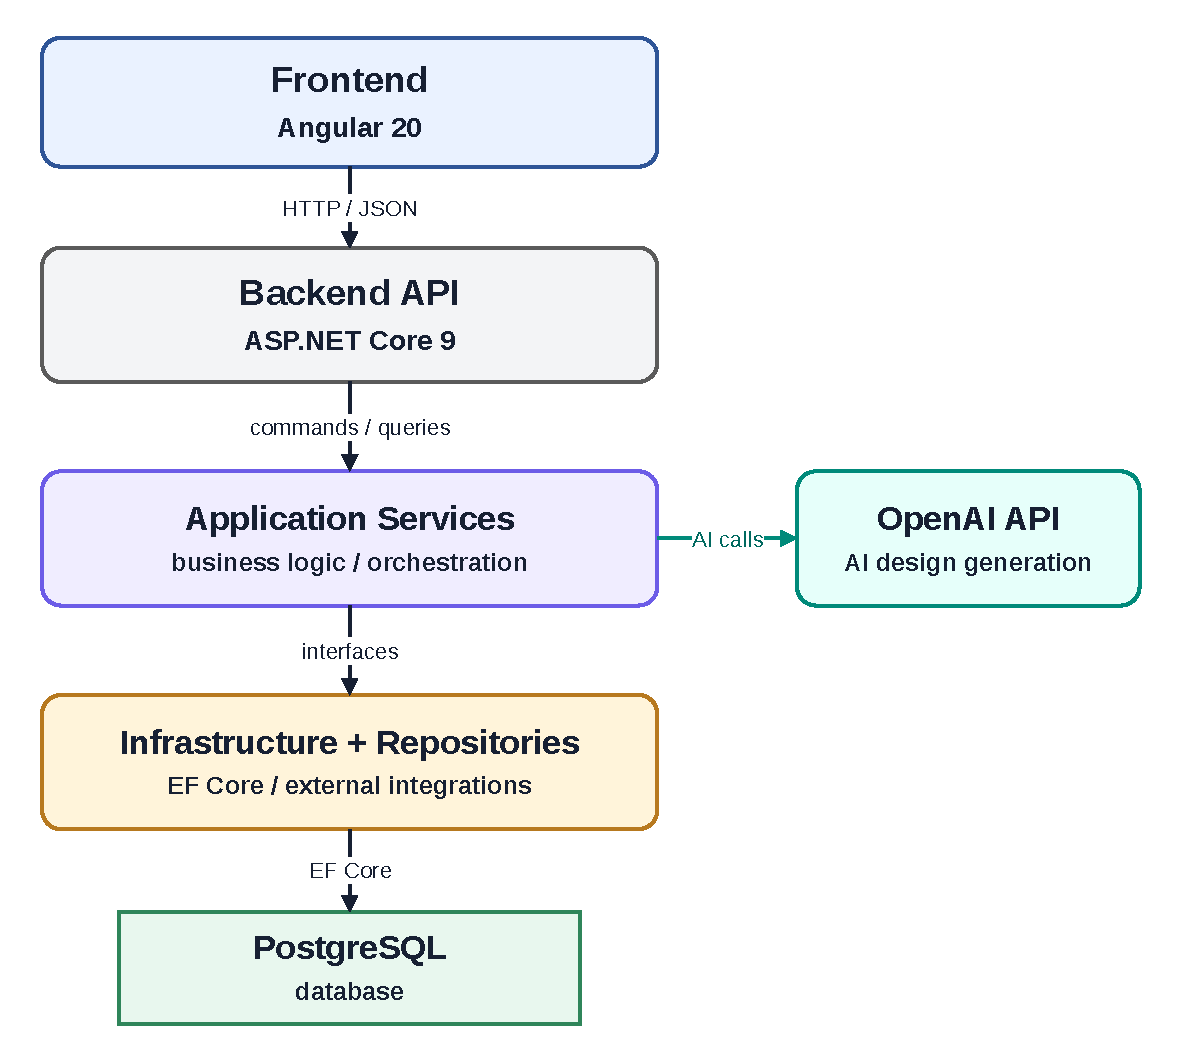
\includegraphics[width=0.92\textwidth]{diagrams/arhitectura-generala.drawio.pdf}
  \caption{Arhitectura logică generală a sistemului}
  \label{fig:arhitectura-generala}
\end{figure}

Această împărțire nu este doar una de prezentare. Ea se regăsește concret în structura soluției backend: proiectele `Favigon.API`, `Favigon.Application`, `Favigon.Infrastructure`, `Favigon.Domain`, `Favigon.Converter` și `Favigon.Tests`. Fiecare are un rol clar, iar motorul de conversie este separat explicit deoarece are propriile reguli și propria logică de transformare.

\section{Organizarea backend-ului pe straturi}

La nivel de backend, fluxul tipic al unei cereri este:

\begin{enumerate}[leftmargin=1.5cm]
  \item controller-ul primește cererea HTTP și verifică aspectele de intrare;
  \item serviciul de aplicație aplică logica de business;
  \item repository-ul sau adaptorul extern execută persistența sau integrarea necesară;
  \item rezultatul este mapat și întors către client.
\end{enumerate}

Această structură reduce riscul ca un controller să devină prea încărcat. De exemplu, un endpoint din `ProjectsController` nu decide singur cum se construiește un slug, cum se șterg asset-urile sau cum se tratează un fork. Toate acestea sunt delegate către `ProjectService`, care la rândul lui colaborează cu repository-ul și cu storage-ul pentru assets.

Avantajul acestei structuri este vizibil și în testare. Pentru că serviciile sunt relativ bine delimitate, ele pot fi verificate independent de transportul HTTP. De aceea, în proiect există teste directe pentru `AuthService`, `ProjectService`, `UserService` și `ConverterEngine`, nu doar teste la nivel de controller.

Aceeași organizare poate fi interpretată și printr-o lentilă apropiată de \textit{clean architecture}. Regulile esențiale ale produsului și reprezentările interne trebuie să rămână în centru, iar infrastructura, transportul HTTP și integrarea cu servicii externe trebuie să depindă de acest nucleu, nu invers. Figura~\ref{fig:clean-backend} sintetizează această idee pentru backend-ul Favigon.

\begin{figure}[H]
  \centering
  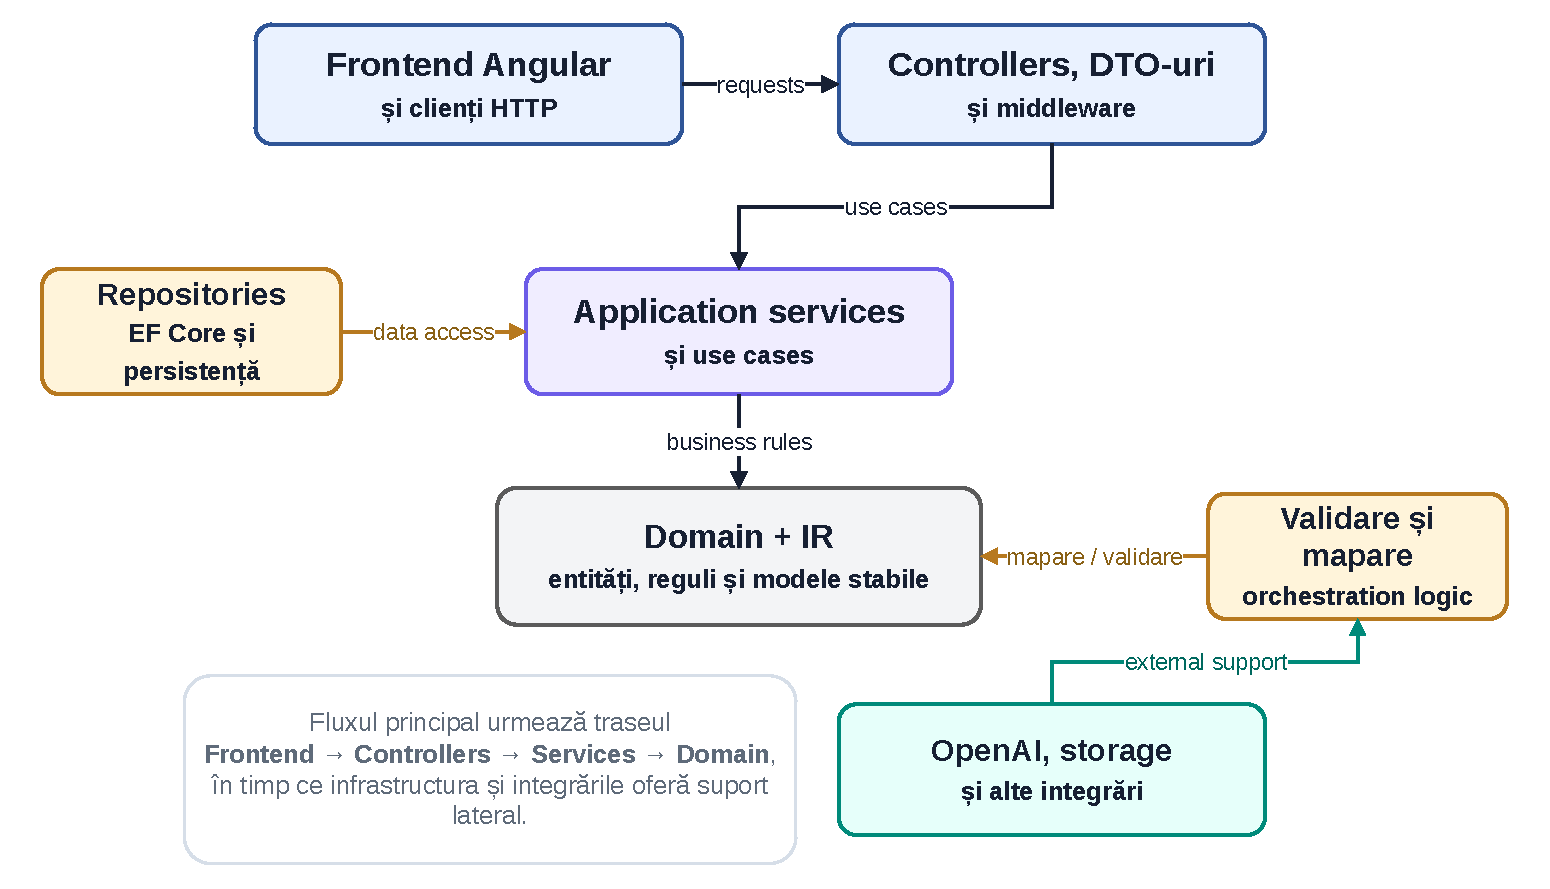
\includegraphics[width=0.95\textwidth]{diagrams/clean-backend.drawio.pdf}
  \caption{Vedere de tip clean architecture pentru backend-ul Favigon}
  \label{fig:clean-backend}
\end{figure}

\section{Organizarea frontend-ului pe feature-uri}

Frontend-ul este organizat în jurul conceptelor `core`, `shared` și `features`. `core` conține modelele, serviciile API, interceptorii și utilitarele globale. `shared` conține componente reutilizabile. `features` grupează zonele funcționale ale aplicației: autentificare, canvas, explore, profil, settings și stars.

Această structură este potrivită pentru proiect deoarece cea mai mare complexitate este concentrată într-un singur feature, anume `canvas`. În loc să împrăștii logica editorului în toată aplicația, serviciile, mapper-ele și utilitarele specifice au fost păstrate aproape de acest feature. În practică, această alegere a redus numărul de dependențe surpriză și a făcut fluxul de lucru mai ușor de urmărit.

\section{Modelul de date conceptual}

Din punct de vedere conceptual, modelul de date are câteva entități centrale: utilizatorul, proiectul, conturile externe legate de utilizator, relațiile de follow dintre utilizatori și relațiile de like sau bookmark dintre utilizatori și proiecte. Designul efectiv al unui proiect este stocat ca JSON în cadrul proiectului, deoarece structura lui este prea flexibilă pentru o modelare exclusiv relațională. Vederea conceptuală simplificată apare în Figura~\ref{fig:model-conceptual}.

\begin{figure}[H]
  \centering
  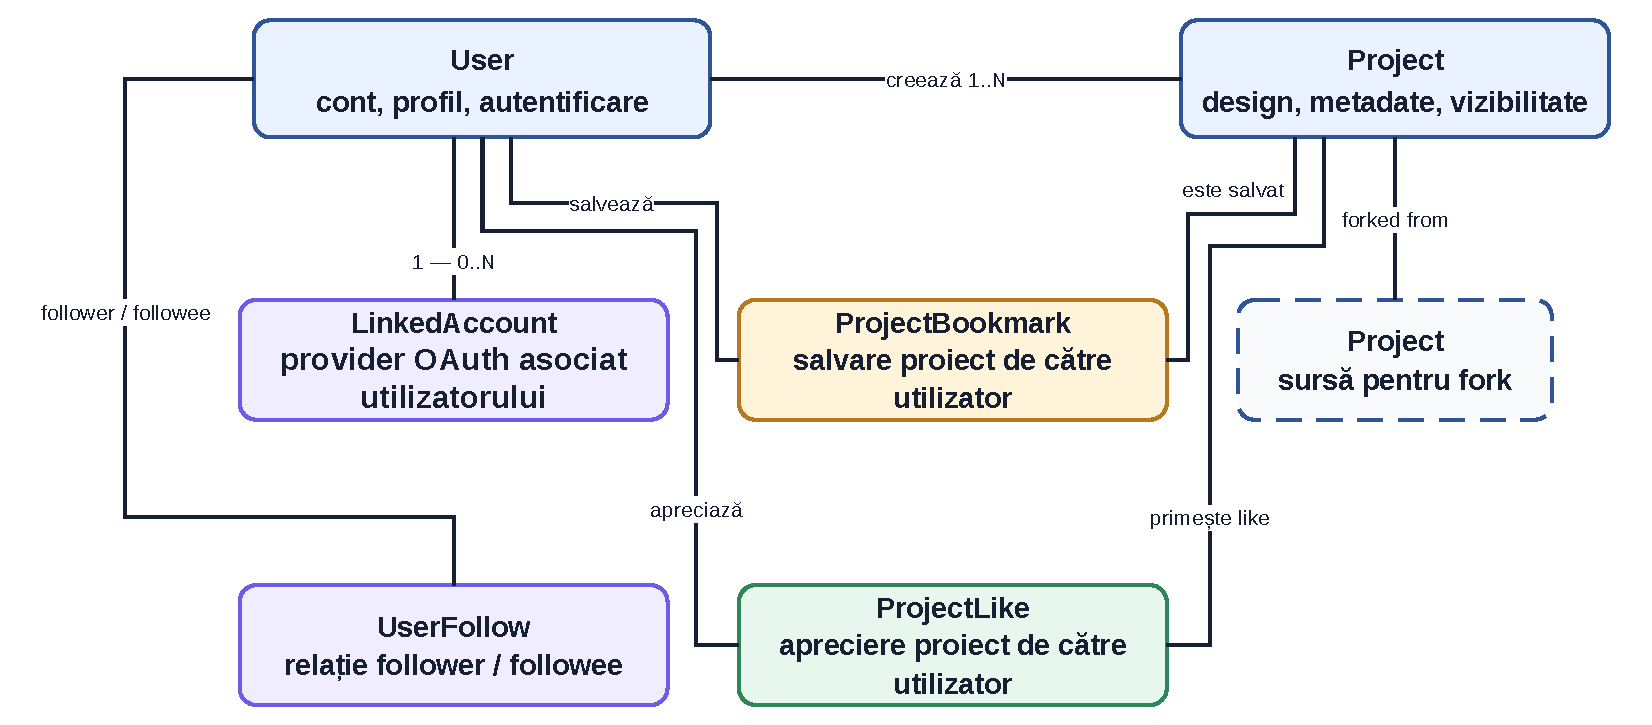
\includegraphics[width=0.94\textwidth]{diagrams/model-conceptual.drawio.pdf}
  \caption{Model conceptual simplificat al datelor principale}
  \label{fig:model-conceptual}
\end{figure}

Din cod se observă și câteva decizii importante. Proiectul are câmpuri pentru `Slug`, `IsPublic`, `ThumbnailDataUrl`, `ViewCount` și `ForkedFromProjectId`. Utilizatorul are câmpuri pentru `HasPassword`, `IsTwoFactorEnabled`, datele de resetare a parolei și date temporare pentru fluxul 2FA. Aceste câmpuri arată că modelul este orientat clar spre un produs complet, nu doar spre stocarea unui desen.

Pentru a trece de la nivelul de domeniu la nivelul de implementare, Figura~\ref{fig:erd-fizic} prezintă un ERD simplificat extras din configurația Entity Framework Core. El evidențiază entitățile persistente, cheile principale și relațiile care merită discutate la nivel de licență.

\begin{figure}[H]
  \centering
  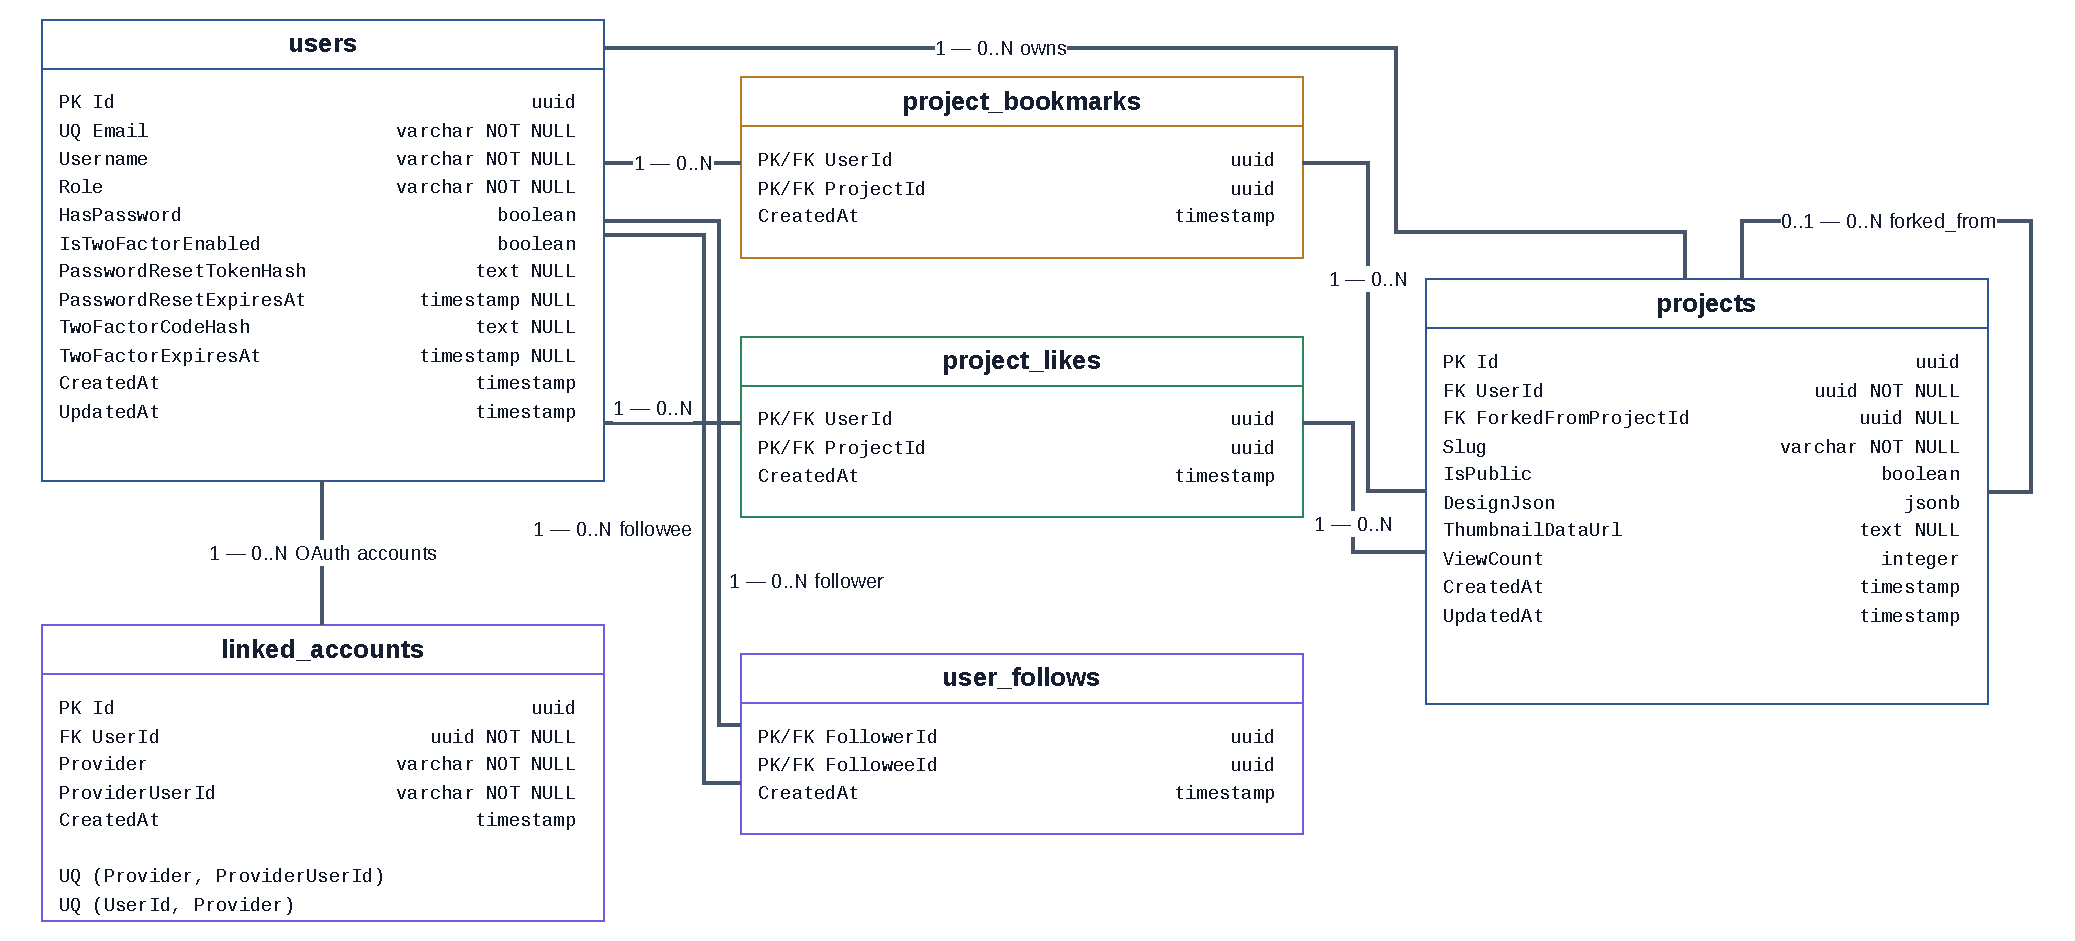
\includegraphics[width=\textwidth]{diagrams/erd-fizic.drawio.pdf}
  \caption{ERD simplificat pentru schema fizică a bazei de date}
  \label{fig:erd-fizic}
\end{figure}

ERD-ul scoate în evidență și câteva constrângeri importante din implementare: unicitatea email-ului pentru utilizatori, unicitatea conturilor externe pe perechile \texttt{(Provider, ProviderUserId)} și \texttt{(UserId, Provider)}, cheile compuse pentru relațiile sociale și autoreferința \texttt{ForkedFromProjectId} din \texttt{projects}. Astfel, schema nu stochează doar resurse izolate, ci și legăturile necesare pentru reutilizare, explorare și trasabilitatea fork-urilor.

Această structură arată explicit și compromisul de modelare adoptat în proiect. Datele cu structură stabilă, cum sunt identitatea utilizatorului, relațiile sociale și metadatele proiectelor, rămân relaționale. În schimb, documentul efectiv al interfeței este păstrat compact în \texttt{DesignJson}, deoarece arborele de elemente, stiluri și layout-uri este prea flexibil pentru a fi mapat eficient în tabele relaționale fine. În plus, timestamp-urile \texttt{CreatedAt} și \texttt{UpdatedAt} sunt menținute automat în contextul de persistență, ceea ce reduce riscul de inconsistență între creare, actualizare și export ulterior.

\section{Fluxurile principale}

\subsection{Fluxul de autentificare}

Fluxul de autentificare începe cu un request către `AccountController`, este procesat în `AuthService`, iar la final backend-ul emite cookie-urile necesare. Dacă utilizatorul are 2FA activ, autentificarea este împărțită în două etape: validarea credențialelor și validarea codului temporar. Această separare este reflectată și în cod, prin token-ul temporar specific fluxului 2FA.

\subsection{Fluxul de editare}

La deschiderea unui proiect, frontend-ul încarcă datele proiectului și apoi designul asociat. `CanvasPersistenceService` coordonează persistarea automată și sincronizarea thumbnail-ului, iar starea editorului este împărțită între mai multe servicii specializate. Din punct de vedere al utilizatorului, totul ar trebui să pară unitar. Din punct de vedere intern, însă, fluxul este descompus în pași mai mici tocmai pentru a păstra controlul asupra lui.

\subsection{Fluxul de export}

Pentru export, editorul produce reprezentarea intermediară, apoi o trimite către backend prin `ConverterController`. `ConverterService` validează structura și apelează `ConverterEngine`, care generează fișierele pentru framework-ul ales. Acest flux este important deoarece justifică separarea convertorului într-un proiect distinct.

\subsection{Fluxul AI}

Pentru generare, frontend-ul trimite un prompt către `AiDesignController`. Backend-ul poate răspunde fie clasic, fie prin streaming SSE. În spate, `AiPipelineService` parcurge fazele de intenție, structură și stil, iar rezultatul final este transformat în date pe care frontend-ul le poate integra în editor.

\section{Decizii de proiectare care au influențat cel mai mult implementarea}

Privind retrospectiv, există câteva decizii de proiectare care au avut impact major asupra întregului proiect.

Prima decizie a fost separarea clară între canvas și codul final exportat. O abordare bazată pe editarea directă a HTML-ului sau a DOM-ului ar fi produs probabil un sistem mai fragil și mai greu de extins.

A doua decizie a fost tratarea AI-ului ca pe un subsistem controlabil, nu ca pe o cutie neagră. De aici rezultă atât folosirea JSON Schema, cât și împărțirea pipeline-ului.

A treia decizie a fost păstrarea logicii editorului în servicii specializate. Fără acest pas, componenta principală de canvas ar fi devenit foarte repede imposibil de întreținut.

A patra decizie a fost folosirea unei baze relaționale pentru metadate și a unui câmp JSON pentru design. Deși este un compromis, el s-a dovedit eficient pentru tipul de informații gestionate.

\section{Concluzii intermediare}

În urma analizei și proiectării, sistemul rezultat are o formă coerentă atât la nivel de produs, cât și la nivel tehnic. Cerințele au fost traduse într-o arhitectură cu straturi clare, actori bine definiți, fluxuri importante și un model de date adaptat problemei.

Capitolul următor trece de la această vedere de ansamblu la implementarea concretă a platformei: autentificare, proiecte, funcții sociale și editorul canvas.







